\documentclass{sig-alternate}

\usepackage{epsfig}
\usepackage{graphicx}
%\usepackage{fancybox}
\usepackage{amssymb}
%\usepackage{stmaryrd}
%\usepackage{a4wide}
%\usepackage{subfigure}
%\usepackage[noend]{algorithmic}
%\usepackage{algorithm}
%\usepackage{listings}
%\usepackage{moreverb}
%\usepackage{boxedminipage}
%\usepackage{algorithm2e}
%\def\floatpagefraction{0.99}
%\linespread{0.99}
%\usepackage{multirow}
%\usepackage{subtable}
%\usepackage{rotating}
\usepackage{subfigure}

%\usepackage[noend]{algcompatible}

\begin{document}
%
% --- Author Metadata here ---
\conferenceinfo{XXX 2012}{City}
\CopyrightYear{2012} % Allows default copyright year (20XX) to be over-ridden - IF NEED BE.
%\crdata{0-12345-67-8/90/01}  % Allows default copyright data (0-89791-88-6/97/05) to be over-ridden - IF NEED BE.
% --- End of Author Metadata ---

\title{X?Name?X: Efficient Execution of Hierarchical Pipelines on Heterogeneous Platforms}
\sloppy

%\numberofauthors{1} %  in this sample file, there are a *total*
%% of EIGHT authors. SIX appear on the 'first-page' (for formatting
%% reasons) and the remaining two appear in the \additionalauthors section.
%%
%\author{
%\alignauthor
%George Teodoro, Tony Pan, Tahsin M. Kurc, Lee Cooper, Jun Kong, and Joel H. Saltz\\
%\affaddr{Center for Comprehensive Informatics}\\
%\affaddr{Emory University}\\
%\affaddr{Atlanta, GA 30322}\\
%\email{\{george.teodoro,tony.pan,tkurc,lee.cooper,jun.kong,jhsaltz\}@emory.edu}
%}
\maketitle
\begin{abstract}
%
abstract.
%
\end{abstract}

\section{Motivation/Objective}

The successful introduction of accelerators as general purpose processors is
changing current High Performance Computing (HPC) systems, which are nowadays
being deployed as heterogeneous CPU-GPU equipped platforms. Taking advantage of
those solutions, however, still be a very hard programming task, mainly due to
the lack of high level programming languages, and runtime frameworks to
abstract the complex interactions among applications and heterogeneous systems.
While some work has been done in order to execute simple kernel applications
using CPUs and GPUs cooperatively, including MapReduce computations for shared
memory machines~\cite{mars,merge,qilin09luk}, the execution of more complex
real world pipelined applications (e.g. with dependency among stages) in
distributed environments still a challenging open problem. The goal of this
work is to propose and implement runtime support to make easier/viable the
deployment of real complex applications on distributed environments. To
accomplish this tasks we will automate/hide from the user most of the complex
tasks regarding interactions of the application with the executing platform,
and provide a set of non-trivial optimizations/scheduling mechanisms.

\section{Runtime System Overview}


Briefly, the runtime system we are building will execute dataflow applications
with dependency among stages, utilizing distributed CPU-GPU equipped platforms.
The overall execution model is based on a bag of tasks, where tasks are
instantiations of a given stage of the application dataflow --- the pair input
data and stage processing functions. To guarantee correct ordering in the
execution of such tasks, the runtime system will use task dependency
information given as input by the user through a simple API, and will assert
that a tasks is not dispatched for execution before all dependencies are
solved. 


%\subsection{Overview}


\begin{figure}[ht]
\begin{center}
\includegraphics[width=0.47\textwidth]{images/appDataflow}
\caption{Sample Application Dataflow.}
\label{fig:sampleDataflow}
\end{center}
\end{figure}

Further, communication among the pipeline stages, or tasks, is performed
through a distributed file system, meaning that data is read and written to
files between stages. Figure~\ref{fig:sampleDataflow} presents a schema of the
multiple levels that may be used to represent a dataflow in this model. In the
first level, Abstract Dataflow, we simply have the logical stages of the
application, describing their connections. In the second level, there is the
instantiation of the dataflow, where the logical computing stages are
associated to different input data, and dependencies among instantiation of
stages (Tasks) are described. For instance, in the left side, there is an
instantiation of the dataflow with an independent replication of the entire
pipeline for each input data.  In the right side, however, there is a more
complex interaction in the dataflow as each input data is computed in parallel
in through multiple instantiations of first stage, but the following stages on
the pipeline will use results computed from the previous instantiations of
stage A (A.1 and A.2). On the bottom level of the same figure, we show that
each logical stage of the application may again be another pipeline, with
dependencies among sub-stages that may additionally have implementation for
multiple devices, e.g. CPU or/and GPU. 

Providing a stage with the capabilities of being described as a pipeline of
multiple sub-tasks has to be (i) with the need of exporting operations with
different performance to the local scheduler (described latter, but similar to
IPDPS), and (ii) with necessity of providing an efficient way for the
application to execute a number of sub-stages without having to write the
output of each of them to the file system, as is necessary in the
communication among stages of the application pipeline.



\begin{figure}[ht]
\begin{center}
\includegraphics[width=0.47\textwidth]{images/executionModel}
\caption{Overview of the system architecture, and task mapping.}
\label{fig:execModel}
\end{center}
\end{figure}

Figure~\ref{fig:execModel} shows the runtime system design, with an overview of
the interaction among its components. In this system, the \emph{Manager} is the
process responsible for handling dependencies among different instantiations of
the dataflow stages (Tasks) (middle level of Figure~\ref{fig:sampleDataflow}),
and to dispatch those tasks for execution with the \emph{Workers}. The
\emph{Workers} will communicate with the \emph{Manager} to request tasks to
compute, retrieve those tasks, and executed them. Each task will read data from
a file system and may spawn a pipeline of sub-tasks that is locally scheduled
by each \emph{Worker}.  When all sub-tasks of a given task are computed, the
\emph{Worker} informs the \emph{Manager}, which may assign another task for
execution. In practice, a single worker may execute multiple Stages, even
concurrently, and both sets of workers presented in Figure~\ref{fig:execModel}
are not necessarily disjoint. 


\begin{figure}[ht]
\begin{center}
\includegraphics[width=0.47\textwidth]{images/worker-environment}
\caption{Workers Environment: the workers is a multi-thread process that may
take advantage of all processing elements in a node to execute the
applications' tasks.}
\label{fig:workerEnv}
\end{center}
\end{figure}

The environment of each Worker, shown in Figure~\ref{fig:workerEnv}, is similar
to what we proposed for IPDPS, with addition of a few features. As discussed,
task dependency management has been added, as well as the communication layer
module that is coupled to abstract exchange of information with the
\emph{Manager}.






\section{Runtime Scheduling}

In addition to building the runtime system infra-structure described in last
section, it will be necessary to provide a hierarchical scheduling to assign
task from the \emph{Manager} to the \emph{Workers}, called Manager Level
Scheduling, as well as internally to each \emph{Worker} --- Worker Level Scheduling. 

\subsection{Manager Level Scheduling}

The main objective is to assign tasks to \emph{Workers} in order to optimize
the performance of the overall system. There are two major aspects that should
be considered:~(i)~Load imbalance among \emph{Workers}, and a demand-driven
task assignment among Workers and Manager should be enough for solving this
problem; (ii)~A smarter choice of which task to assign for a Worker could also
potentially improve the performance. For instance, if a Worker already has a
number of tasks with low speedup, it would be better to sent a task with high
speedup for that Worker, which may be able to make better local scheduling
decisions. This tends to be better than traditional FCFS scheduling, as we
observed in the PRIORITY compared to FCFS.  Below is the list of features that
should be added to the Manager scheduler.

\begin{itemize}
	\item Demand-driven tasks assignment;

	\item Multi-task assignment to overlap communication/computation;

	\item Performance Aware task choice;
\end{itemize}

\subsection{Worker Level Scheduling}

The Worker level scheduler is more aligned with what we already proposed for 
the IPDPS paper, with addition of dependency among tasks, and potentially new
scheduling techniques that take into account the number of dependencies when
choosing a task to executed. The summary of features is:

\begin{itemize}
	\item Support to dependency among sub-tasks;

	\item Scheduling policies similar to those described in~\cite{Teodoro-IPDPS2012};

	\item May include number of tasks dependencies into the scheduling decision;

\end{itemize}


\subsection{Analytical Performance Model}

\begin{itemize}

	\item Set of tools to analytically estimate applications' performance.
We already have a draft that we intended to use with the HPDC, before it turn
into Morphological Reconstruction;

\end{itemize}



\input{learning}

\section{Other related work}

These are some frameworks we should mention in the related
work~\cite{6061070,LEMENTEC:2011:HAL-00648245:1,ravi2010compiler}


%\end{document}  % This is where a 'short' article might terminate

%ACKNOWLEDGMENTS are optional
%\section{Acknowledgments}
%This section is optional; it is a location for you
%to acknowledge grants, funding, editing assistance and
%what have you.  In the present case, for example, the
%authors would like to thank Gerald Murray of ACM for
%his help in codifying this \textit{Author's Guide}
%and the \textbf{.cls} and \textbf{.tex} files that it describes.

%
% The following two commands are all you need in the
% initial runs of your .tex file to
% produce the bibliography for the citations in your paper.
\bibliographystyle{abbrv}
\bibliography{george}  % sigproc.bib is the name of the Bibliography in this case
% You must have a proper ".bib" file
%  and remember to run:
% latex bibtex latex latex
% to resolve all references
%

%\balancecolumns % GM June 2007
% That's all folks!
\end{document}
